\section{Tiền xử lý dữ liệu (Data Preprocessing)}
\label{sec:c}

\subsection{Nguyên tắc và kiểm soát rò rỉ}
Phương án xử lý chỉ dựa trên các phát hiện của Phần A (chỉ đọc D3). Script \var{03_preprocess.py} chỉ có một lệnh đọc dữ liệu, nằm trong hàm kiểm tra đường dẫn chỉ cho phép D3 và data dictionary;
nghiệm thu còn quét mã nguồn để bảo đảm không chứa tên D0--D2 hay thư mục dữ liệu ẩn. Sau khi 15/15 kiểm tra nghiệm thu đạt, bốn file kết quả được ghi mã băm SHA-256 và khóa ghi;
script đối chiếu \var{03b_evaluate_preprocessing.py} từ chối chạy nếu mã băm lệch (đã thử: sửa 1 byte thì bị từ chối). Chỉ sau đó D0 mới được mở, và chỉ để tính số đo tổng hợp, \emph{không} dùng để thay thế từng giá trị.
Đầu ra giữ nguyên đơn vị và độ chính xác gốc; log, chuẩn hóa và mã hóa được thực hiện ở bước chuẩn bị dữ liệu (mục~\ref{sec:d}).

\subsection{Phương án xử lý và cơ sở}
\begin{table}[htbp]
\centering\small
\caption{Quyết định tiền xử lý. Mọi cơ sở lấy từ D3; mọi thay đổi ghi vào nhật ký từng ô (72 ô).}
\label{tab:cdecisions}
\begin{tabularx}{\linewidth}{>{\raggedright\arraybackslash}p{2.6cm}>{\raggedright\arraybackslash}X>{\raggedright\arraybackslash}X}
\toprule
Vấn đề & Quyết định & Cơ sở và phương án đã loại\\
\midrule
7 ô không hợp lệ & Giữ nguyên dòng; vô hiệu hóa \emph{từng ô} (6 vi phạm luật miền, 1 vi phạm đẳng thức) rồi điền. &
Mỗi dòng chỉ hỏng một ô, 13 ô còn lại hợp lệ. Loại: xóa dòng; cắt ngưỡng (tạo điểm dồn giả ở biên).\\
Dòng C0062 (AOV 3\,093 so với total$/n$ = 40,04) & Vô hiệu hóa ô AOV và điền bằng mô hình như mọi ô khác; \textbf{không} gán $\mathrm{AOV}=\mathrm{total}/n$. &
Data Dictionary ghi $\mathrm{total}\sim n\times\mathrm{AOV}$ (xấp xỉ), không xác nhận đẳng thức chính xác, và sd bền của độ lệch đẳng thức ở dòng bình thường là $0{,}164$ ($\approx 16\%$). Ô nghi chọn theo phân vị biên: AOV 99,6\%, total 60,8\%, $n$ 59,2\%; hạng bronze khớp với total thấp.\\
Giá trị thiếu (số) & Chọn phương pháp điền theo thí nghiệm che ô (Bảng~\ref{tab:imp}). & Trung vị toàn cục tạo 22--32 giá trị trùng; xóa dòng mất 23,5\%.\\
\var{preferred_category} & Giữ mức \texttt{unknown}; các biến thể KNN-7/mode được lưu riêng để so sánh (Bảng~\ref{tab:sens}). &
Độ chính xác che ô tốt nhất $0{,}40$ nên nhãn điền vào sai nhiều hơn đúng (mục~\ref{sec:c_cat}).\\
Nhiễu & \textbf{Không khử nhiễu từng giá trị}; không làm mượt, không winsorize. &
Nhiễu độc lập từng ô không phục hồi được từ D3; làm mượt trộn khách khác nhóm và co các hồ sơ hiếm; winsorize tạo điểm dồn.\\
Cực trị hợp lệ & Chỉ ghi cờ (34 dòng, 56 ô ngoài 3 IQR và không vi phạm luật nào), không sửa, không xóa. &
Tukey $1{,}5$ IQR gắn cờ 94 dòng với precision $0{,}14$; xóa sẽ loại nhóm khách giá trị cao thật.\\
Điểm dồn ở biên & Giữ nguyên, ghi cờ; không ô nào được điền rơi đúng giá trị biên. &
Thấy ngay trong D3: \var{sessions_per_month}=0,5 (12 dòng), \var{recency_days}=0 (15), =365 (11), \var{n_orders_12m}=1 (80), \var{age}=18 (22). Jitter là bịa dữ liệu.\\
\bottomrule
\end{tabularx}
\end{table}

\subsection{Chọn phương pháp điền khuyết}
Với mỗi cột cần điền, 15\% ô \emph{đã quan sát} bị che ngẫu nhiên, lặp 50 lần với \textbf{cùng một tập mask cho mọi phương pháp} (so sánh ghép cặp); năm phương pháp được đo bằng MAE ở đơn vị gốc. Quy tắc 1-SE: chọn phương pháp \emph{đơn giản nhất}
(thứ tự trung vị $<$ trung vị theo thiết bị $<$ KNN5 $<$ KNN10 $<$ hồi quy lặp) có MAE không vượt MAE tốt nhất cộng một sai số chuẩn của nó. Với \var{age} sai số được báo bằng năm.

\begin{table}[htbp]
\centering\small
\caption{Thí nghiệm che ô: MAE trung bình (độ lệch chuẩn qua 50 lần; sai số chuẩn SE). In đậm là phương pháp được chọn.}
\label{tab:imp}
\begin{tabular}{lcc}
\toprule
Phương pháp & \var{age} (năm; 36 ô/lần) & \var{avg_session_minutes} (phút; 34 ô/lần)\\
\midrule
Trung vị toàn cục & 8,82 (0,84; SE 0,118) & 7,69 (1,41; SE 0,200)\\
Trung vị theo thiết bị & 8,13 (0,82; SE 0,116) & 7,65 (1,42; SE 0,200)\\
KNN ($k=5$) & 7,10 (0,89; SE 0,126) & 4,10 (0,95; SE 0,134)\\
KNN ($k=10$) & \textbf{6,89 (0,86; SE 0,122)} & 4,01 (0,93; SE 0,132)\\
Hồi quy lặp & 7,20 (0,79; SE 0,111) & \textbf{3,04 (0,60; SE 0,085)}\\
\bottomrule
\end{tabular}
\end{table}

Các cột còn lại (mỗi cột chỉ 1 ô cần điền) được chọn theo cùng quy tắc: \var{avg_order_value} và \var{recency_days} dùng hồi quy lặp; \var{discount_usage_rate} và \var{cart_abandon_rate} dùng KNN5;
\var{sessions_per_month} dùng KNN10. Tuổi gần như không đoán được từ các cột khác: KNN10 chỉ giảm MAE khoảng 22\% so với trung vị, nên các ô tuổi điền vào mang rất ít thông tin.

\subsubsection{Vì sao giữ \texttt{unknown} cho \var{preferred_category}}
\label{sec:c_cat}
Quyết định dựa trên mức bất định, không dùng một ngưỡng độ chính xác chung. Che 15\% ô, 50 lần, cùng mask: mode toàn cục đúng $0{,}254$, mode theo thiết bị $0{,}218$, mode theo hạng $0{,}197$, KNN-7 $0{,}402$.
KNN-7 hơn mode toàn cục $0{,}148$ (SE ghép cặp $0{,}013$): tốt hơn thật nhưng vẫn sai khoảng 60\% lần. Trên chính 13 ô thiếu, xác suất lớp dự đoán trung bình chỉ $0{,}53$ (từ $0{,}40$ đến $0{,}71$) và entropy chuẩn hóa $0{,}64$;
kỳ vọng sai khoảng $7{,}8$ trên 13 nhãn nếu điền. Một nhãn gán vào mà xác suất sai lớn hơn xác suất đúng, trên một biến chiếm 5\% dòng, là thông tin bịa thêm; \texttt{unknown} không bịa. Phân tích độ nhạy ở mục~\ref{sec:e} (Bảng~\ref{tab:sens}) cho thấy cách xử lý này không làm thay đổi đáng kể kết quả phân cụm.

\subsection{Kết quả xử lý (chỉ dựa trên D3 và dữ liệu đã xử lý)}
Có 72 ô thay đổi: 7 ô không hợp lệ được điền, 21 ô \var{age} và 31 ô \var{avg_session_minutes} thiếu được điền, 13 ô \var{preferred_category} thành \texttt{unknown}; mọi ô khác giữ nguyên từng giá trị.
Ô AOV của C0062 được điền $40{,}75$, gần total$/n=40{,}04$ (chỉ dùng kiểm tra hợp lý). Trên D3, phần bình phương khoảng cách do 7 dòng đã sửa gây ra giảm từ $0{,}314$ xuống $0{,}041$ (z-score thô) và từ $0{,}152$ xuống $0{,}044$ (log1p + median/IQR) (Hình~\ref{fig:c_struct});
độ lệch chuẩn của \var{sessions_per_month} so với độ lệch chuẩn bền giảm từ $7{,}7$ xuống $1{,}0$, của \var{avg_session_minutes} từ $11{,}1$ xuống $1{,}4$. Điểm dồn ở biên không đổi (12, 15, 11, 80, 22) và không ô điền nào rơi đúng giá trị biên.

\begin{figure}[htbp]
\centering
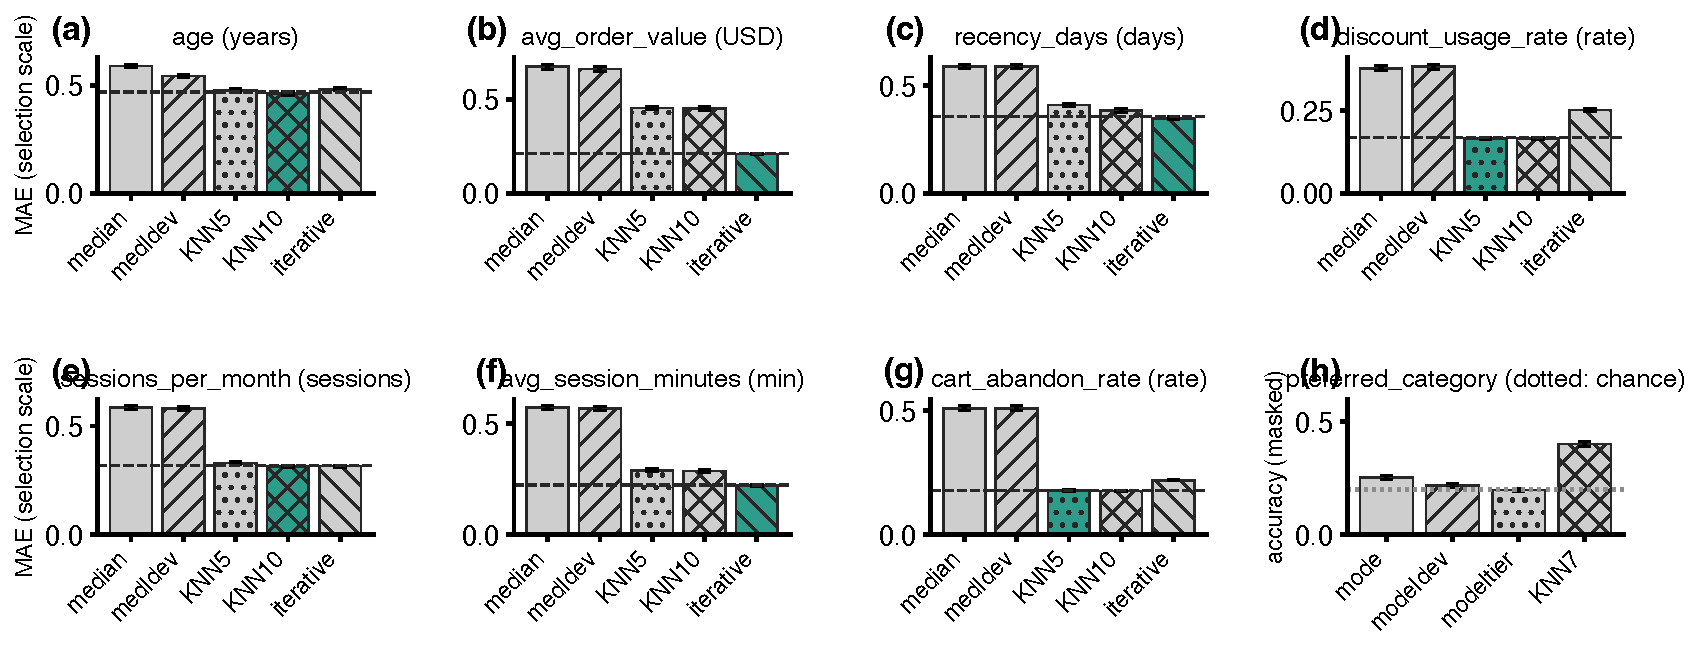
\includegraphics[width=\linewidth]{fig01_imputer_selection.pdf}
\caption{Chọn phương pháp điền: MAE (thang chọn, thanh sai số = SE; số ghi trên cột là MAE theo đơn vị gốc) cho từng cột và độ chính xác che ô của \var{preferred_category} (h).
Màu lam-lục là phương pháp được chọn; đường nét đứt là ngưỡng 1-SE.}
\label{fig:c_select}
\end{figure}

\begin{figure}[htbp]
\centering
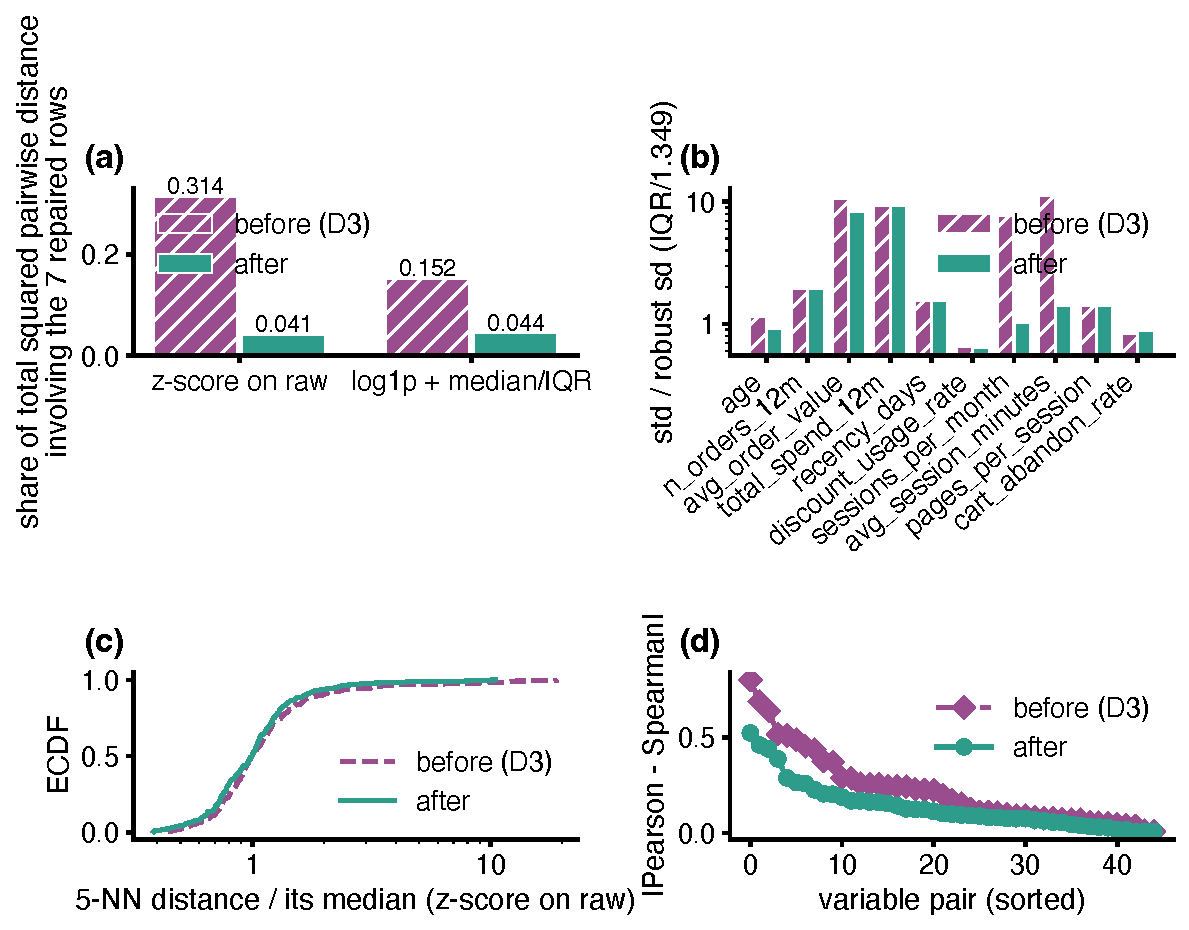
\includegraphics[width=0.92\linewidth]{fig04_structure_before_after.pdf}
\caption{Cấu trúc trước (D3) và sau xử lý, tính chỉ từ D3 và dữ liệu đã xử lý. (a) Phần bình phương khoảng cách liên quan 7 dòng đã sửa. (b) Độ lệch chuẩn chia độ lệch chuẩn bền theo cột.
(c) ECDF khoảng cách láng giềng thứ 5 chuẩn hóa theo trung vị. (d) Chênh lệch $|\text{Pearson}-\text{Spearman}|$ của các cặp biến.}
\label{fig:c_struct}
\end{figure}

\subsection{Đối chiếu với dữ liệu sạch (sau đóng băng)}
Các số đo dưới đây chỉ mô tả mức khớp tổng hợp với D0; chúng \emph{không} phải sai số khôi phục từng ô và không được dùng để chỉnh quy trình.
\begin{table}[htbp]
\centering\small
\caption{Mức khớp cấu trúc với D0 (z-score thô). Trước = D3; Sau = dữ liệu đã xử lý.}
\label{tab:c_eval}
\begin{tabular}{lccc}
\toprule
Số đo & D0 (tham chiếu) & Trước & Sau\\
\midrule
Trung bình $|\Delta$ Pearson$|$ so với D0 & 0 & 0,178 & 0,063\\
Trung bình $|\Delta$ Spearman$|$ so với D0 & 0 & 0,020 & 0,017\\
5-NN giữ lại so với D0 & 1,00 & 0,527 & 0,630\\
Tương quan hạng khoảng cách so với D0 & 1,00 & 0,772 & 0,878\\
Hopkins & 0,833 & 0,940 & 0,885\\
Silhouette theo nhãn ẩn (chẩn đoán) & 0,298 & 0,281 & 0,288\\
\bottomrule
\end{tabular}
\end{table}
\begin{itemize}
\item \textbf{Cải thiện rõ:} tỉ số độ lệch chuẩn với D0 của \var{sessions_per_month} giảm từ $8{,}31$ xuống $1{,}10$, của \var{avg_session_minutes} từ $9{,}07$ xuống $1{,}03$; sai khác Pearson với D0 giảm từ $0{,}178$ xuống $0{,}063$.
Với 31 ô \var{avg_session_minutes} được điền, MAE so với D0 là $2{,}95$ phút (mốc trung vị toàn cục $6{,}23$; sàn nhiễu $|\mathrm{D2}-\mathrm{D0}|$ là $2{,}15$); tương quan với D0 là $0{,}92$.
\item \textbf{Cải thiện khiêm tốn:} 21 ô \var{age} có MAE $7{,}14$ năm (mốc $8{,}24$), tương quan $0{,}58$, và độ phân tán chỉ bằng $0{,}53$ lần giá trị thật (điền đơn trị co phương sai).
\item \textbf{Không cải thiện hoặc xấu đi:} thống kê KS của \var{age} tăng từ $0{,}011$ lên $0{,}023$; KS của \var{sessions_per_month} giữ $0{,}050$ (do điểm dồn ở $0{,}5$); độ lệch của \var{avg_order_value} tăng từ $9{,}19$ lên $10{,}92$
vì các giá trị cực trị hợp lệ còn nguyên; số đo 5-NN chỉ đạt $0{,}63$ vì nhiễu chưa được xử lý.
\item \textbf{Một lần điền sai nhiều:} ô \var{recency_days} của C0242 được điền 210 ngày trong khi D0 là 69 (mốc trung vị toàn cục 26). Tôi không đổi phương pháp sau khi biết kết quả này để tránh rò rỉ từ dữ liệu sạch.
\end{itemize}

\begin{figure}[htbp]
\centering
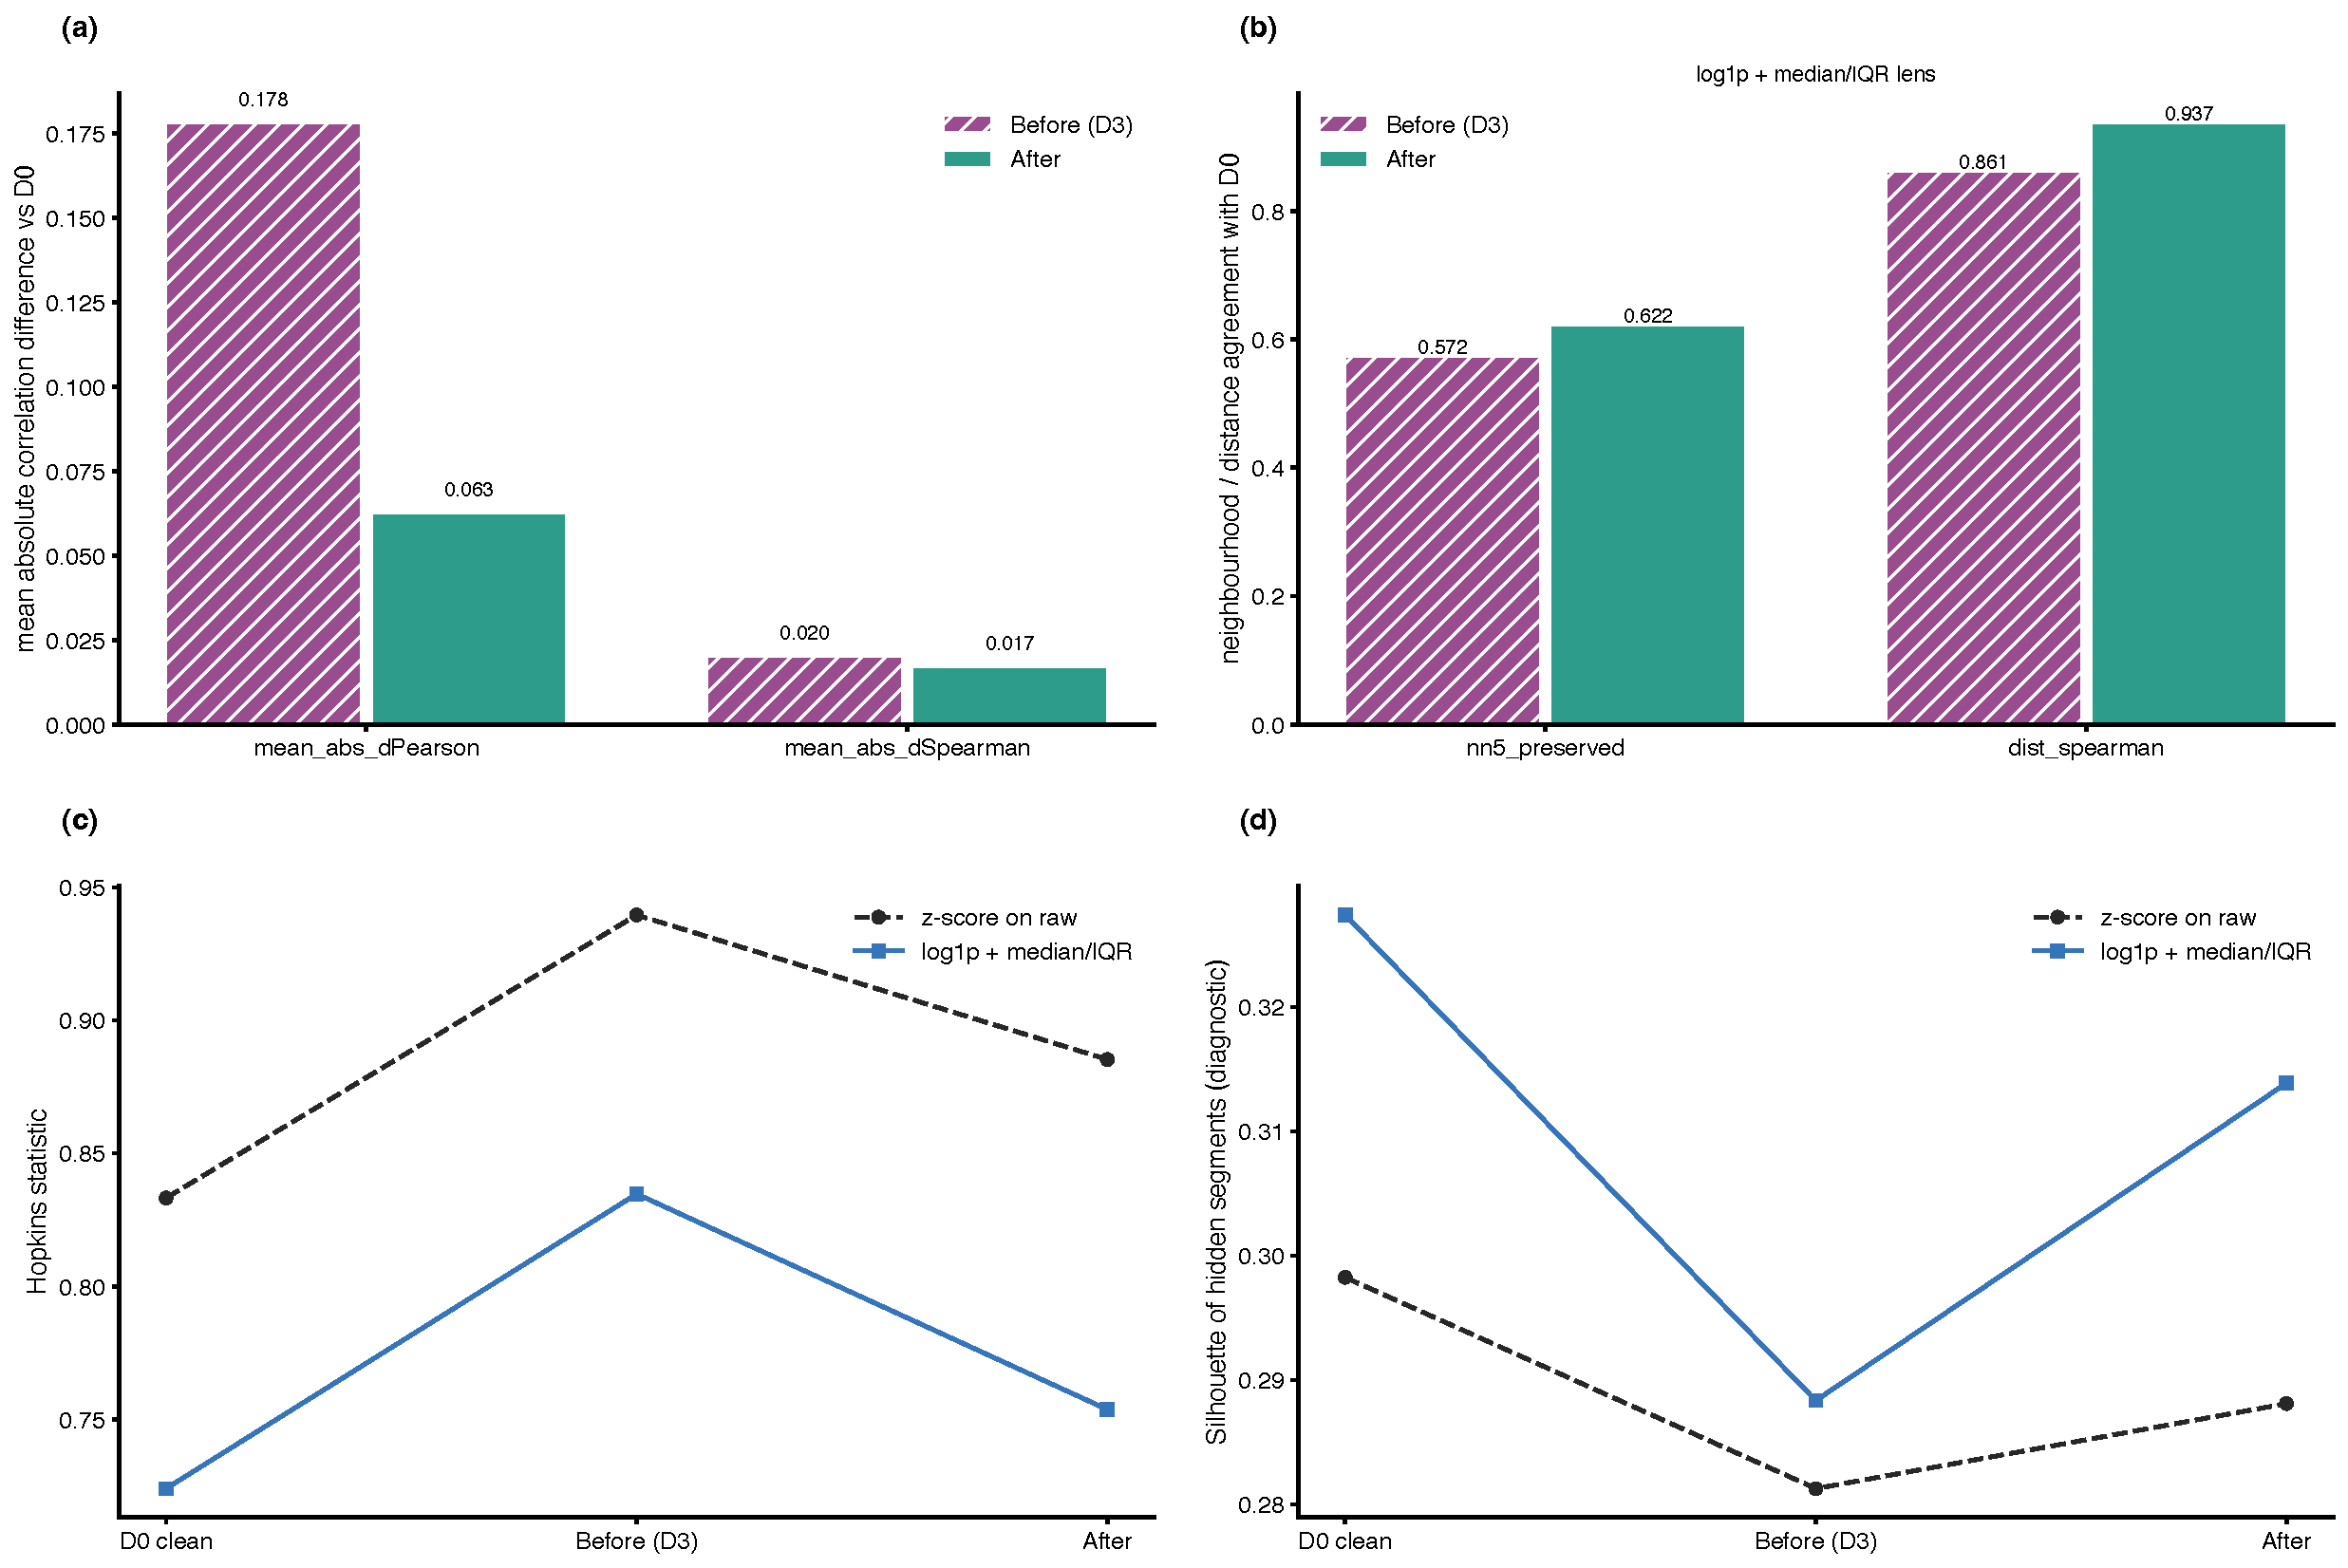
\includegraphics[width=0.92\linewidth]{figE3_structure_vs_clean.pdf}
\caption{Đối chiếu với D0 sau đóng băng (Trước = D3, Sau = đã xử lý). (a) Sai khác tương quan trung bình. (b) Mức giữ lân cận và khoảng cách (log1p + median/IQR).
(c) Hopkins; (d) Silhouette theo nhãn ẩn (chẩn đoán).}
\label{fig:c_eval}
\end{figure}
\FloatBarrier
